The semantics of the combination $\pi$-OZ specification S can then be described by the \picalc{} process $S_{OZ\_part_\pi} \mid S_{\pi\_part}$, where $S_{OZ\_part_\pi}$ is the syntactic transformation of \oz{} part into \picalc{} process. For example, the semantics of \refFig{comp_oz_pi_statefull_vm} is $VM\_OZ\_PI \mid VM\_PI$, where $VM\_OZ\_PI$ is as descriped in \refLis{tra_vm_OZ_listing}. Unfortunately, this will not work well, since the parallel operator $|$ only allows the binary synchronization via a channel, not like in $CSP$ where the parallel operator $||$ allows the multiple synchronization via a channel. That will be problematic when we try to combine the $\pi$-OZ specification of an entity S with a $\pi$-OZ specification of another entity R in parallel. To solve this problem we can use   \textbf{broadcast channel} or  \textbf{non-atomic communication} concepts as follow:

\subsubsection{\findex{Broadcast Channel:}}
To allow the multiple synchronization via a channel in \picalc{}, we use concept of the broadcast channel. \cite{ene} introduces the b$\pi$, which is an extension of \picalc{} implementing broadcast communications. In \cite{olderog08} the UPPAAL model checker introduces the broadcast channel too. For simplicity, we use the concept from \cite{olderog08} for the broadcast channel with a little change. On a broadcast channel one sender synchronize with an at least one receivers. Thus, like binary synchronization, broadcast blocks the sender if there is no receivers. Furthermore, we can send and receive on a broadcast channel. We extend the transition rules of \picalc{} defined in \refDef{def_pi_trans_system}, with an additional rule:
\begin{figure}[H]
\begin{gather*}
\kalRuleM[if\ x: Broadcast]{Broadcast\_Chan\_PAR}{}{P \transs{\out{x}{\vec{y}}} P'}{Q \transs{\inp{x}{\vec{y}}} Q'}{R \transs{\inp{x}{\vec{z}}} R'}{\procpar{\procpar{P}{Q}}{R} \transs{\tau} 
\procpar{P'}{\procpar{\substitue{\vec{y}}{\vec{z}}Q'}{\substitue{\vec{y}}{\vec{z}}R'}}
}
\end{gather*}
\caption{transition rule for broadcast channel.}
\label{fig_broadcast_channel}
\end{figure}



\refFig{comp_oz_pi_statefull_vm_broadcast} shows the $\pi$-OZ specification of our $VM$ using broadcast channels.
The combination's process $S_{OZ\_part_\pi} \mid S_{\pi\_part}$ for $VM$ is $VM\_OZ\_PI \mid VM\_PI$. The main advantage of the broadcast channels in $VM$ is that, if we combine the combination's processes with a third processes $Cus$ representing a customer which issues a signal on the $coffee$ channel, this will enforce both $VM\_OZ\_PI$ and $VM\_PI$ to evolve, since they are listening on coffee , which is broadcast channel in  $Cus$, $VM\_OZ\_PI$ and $VM\_PI$. The behavior of $VM$ can be seen as the intersection of the behavior of  $VM\_OZ\_PI$ and $VM\_PI$ .i.e. the intersection of the transition graphs .i.e the automates. Unfortunately, our tools doesn't support the broadcast channel, thus we will not proceed with this approach.
\begin{figure}[H]
\centering
\begin{class}{VM(id: \integer)}
\ 
\\shared\ chan\ coffee,tea
\ 
\\shared\ chan\ talk:\integer \times \integer
\ \\ \
\\VM\_PI = coffee().VM\_PI + tea().VM\_PI 
\\ \ \qquad \qquad + talk<self,message>.VM\_PI
\\
\begin{state}
self, cv, tv, message: \integer
\ST
0 \leq  cv \leq 3
\\
0 \leq  tv \leq 3
\end{state} 
\\
\begin{init}
self = id
\\cv = 3
\\tv = 3
\\ message= 1
\end{init} 
\\
\begin{op}{coffee}
\Delta (cv)
\ST
cv' = cv - 1
\end{op}
\\
\begin{op}{tea}
\Delta (tv)
\ST
tv' = tv - 1
\end{op}
\\
\begin{op}{talk}
y!: \integer
\\z!: \integer
\ST
y! = message
\\z! = self
\end{op}
\end{class}
\caption{$\pi$-OZ specification of the $VM$ using broadcast channels.}
\label{comp_oz_pi_statefull_vm_broadcast}
\end{figure}



\subsubsection{\findex{Action reproducing and non-atomic reaction}:} Let us examine the process $Cus \mid VM\_OZ\_PI \mid VM\_PI$. When $Cus$ issues a signal on the $coffee$ channel, it is required that $VM\_OZ\_PI$ and $VM\_PI$ receives the signal and evolve together. This is not possible , since the \picalc{} communications are binary, so either $VM\_OZ\_PI$ or $VM\_PI$ will evolve and the other will not. To solve this problem using binary communications we can reproduce the signal. That is , the $Cus$ issues a signal to $VM\_PI$ and waits for a done signal, $VM\_PI$ reproduces the signal and sends it to $VM\_OZ\_PI$ and waits for done signal. When $VM\_OZ\_PI$ ends it sends done signal to $VM\_PI$ which sends done signal to $Cus$. This way the combination's process $S_{OZ\_part_\pi} \mid S_{\pi\_part}$ behaves as a one processes from the view of its environment by reproducing the action and using the done signal, what makes the reaction non-atomic. The implantation of the action reproducing and non-atomic reaction concept requires breaking the channel $coffee$ down into two channels: $ex\_cofee$ and $in\_coffee$. The channel $ex\_cofee$ for the external, outside $VM$, communication between $Cus$ and $VM\_PI$. The channel $in\_coffee$ for the internal, inside $VM$, communication between $VM\_PI$ and $VM\_OZ\_PI$ as shown in \refFig{non_atomic_reactoin}.

\begin{figure}[H]%
\centering
\fbox{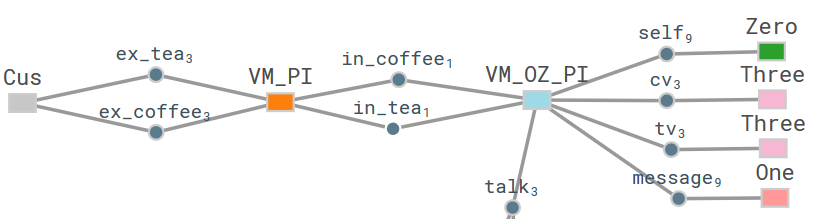
\includegraphics[keepaspectratio,width=0.95\textwidth]{./images/the_compination_pi_oz/non_atomic_reactoin.png}}%
\caption{Action reproducing and non-atomic reaction}
\label{non_atomic_reactoin}%
\end{figure}

\begin{figure}[H]
\centering
\begin{class}{VM(id: \integer)}
\ 
\\chan\ ex\_coffee,in\_coffee,ex\_tea,in\_tea
\ 
\\chan\ talk:\integer \times \integer
\ \\ \
\\VM\_PI = ex\_coffee().in\_coffee<>.VM\_PI 
\\ \ \qquad \qquad + ex\_tea().in\_tea<>.VM\_PI 
\\ \ \qquad \qquad + talk<self,message>.VM\_PI
\\
\begin{state}
self, cv, tv, message: \integer
\ST
0 \leq  cv \leq 3
\\
0 \leq  tv \leq 3
\end{state} 
\\
\begin{init}
self = id
\\cv = 3
\\tv = 3
\\ message= 1
\end{init} 
\\
\begin{op}{in\_coffee}
\Delta (cv)
\ST
cv' = cv - 1
\end{op}
\\
\begin{op}{in\_tea}
\Delta (tv)
\ST
tv' = tv - 1
\end{op}
\\
\begin{op}{talk}
y!: \integer
\\z!: \integer
\ST
y! = message
\\z! = self
\end{op}
\end{class}
\caption{$\pi$-OZ specification of the $VM$ using broadcast channels.}
\label{comp_oz_pi_statefull_vm_broadcast}
\end{figure}
